\documentclass[12pt,letterpaper]{article} %12-point font, US letter size
\usepackage{mathptmx} %Times new roman with math support
\usepackage{fontenc}
\usepackage[english]{babel}

%figures
\usepackage[pdftex]{graphicx} 

\begin{document}

\thispagestyle{empty}

%\begin{figure}[!ht]
%\centering
%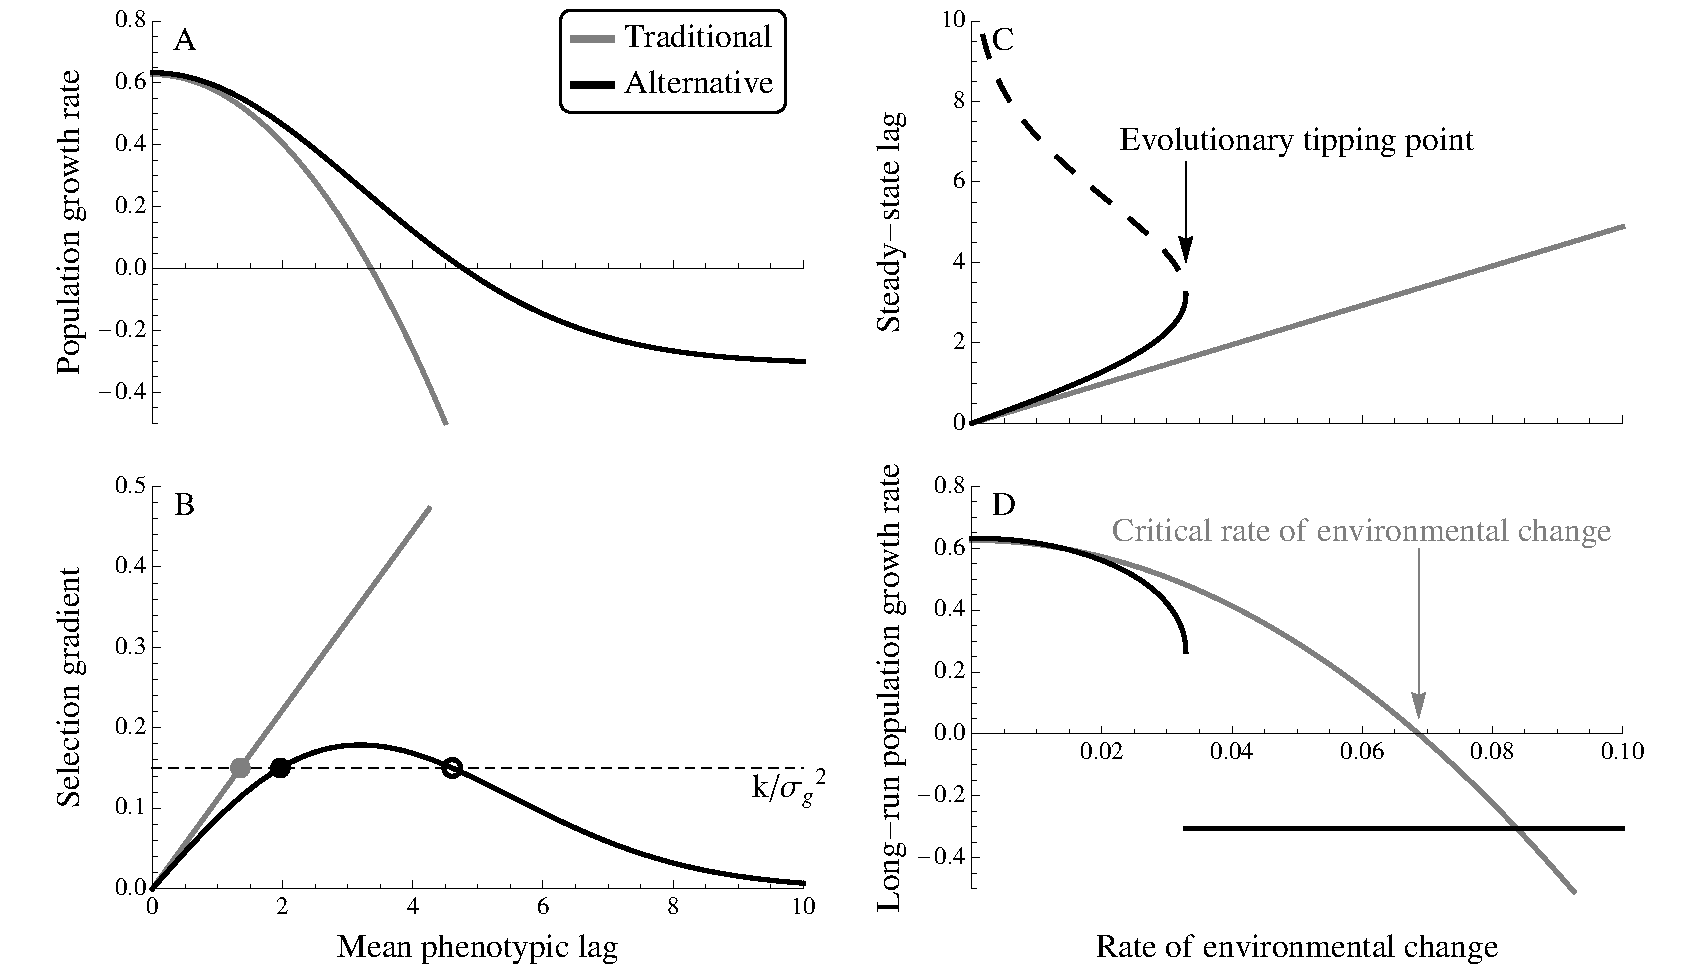
\includegraphics[width=\linewidth]{IMAGES/Didactics}
%\caption{
%}
%\label{SSGrowth}
%\end{figure}

\setcounter{figure}{1}
\begin{figure}[!ht]
\centering
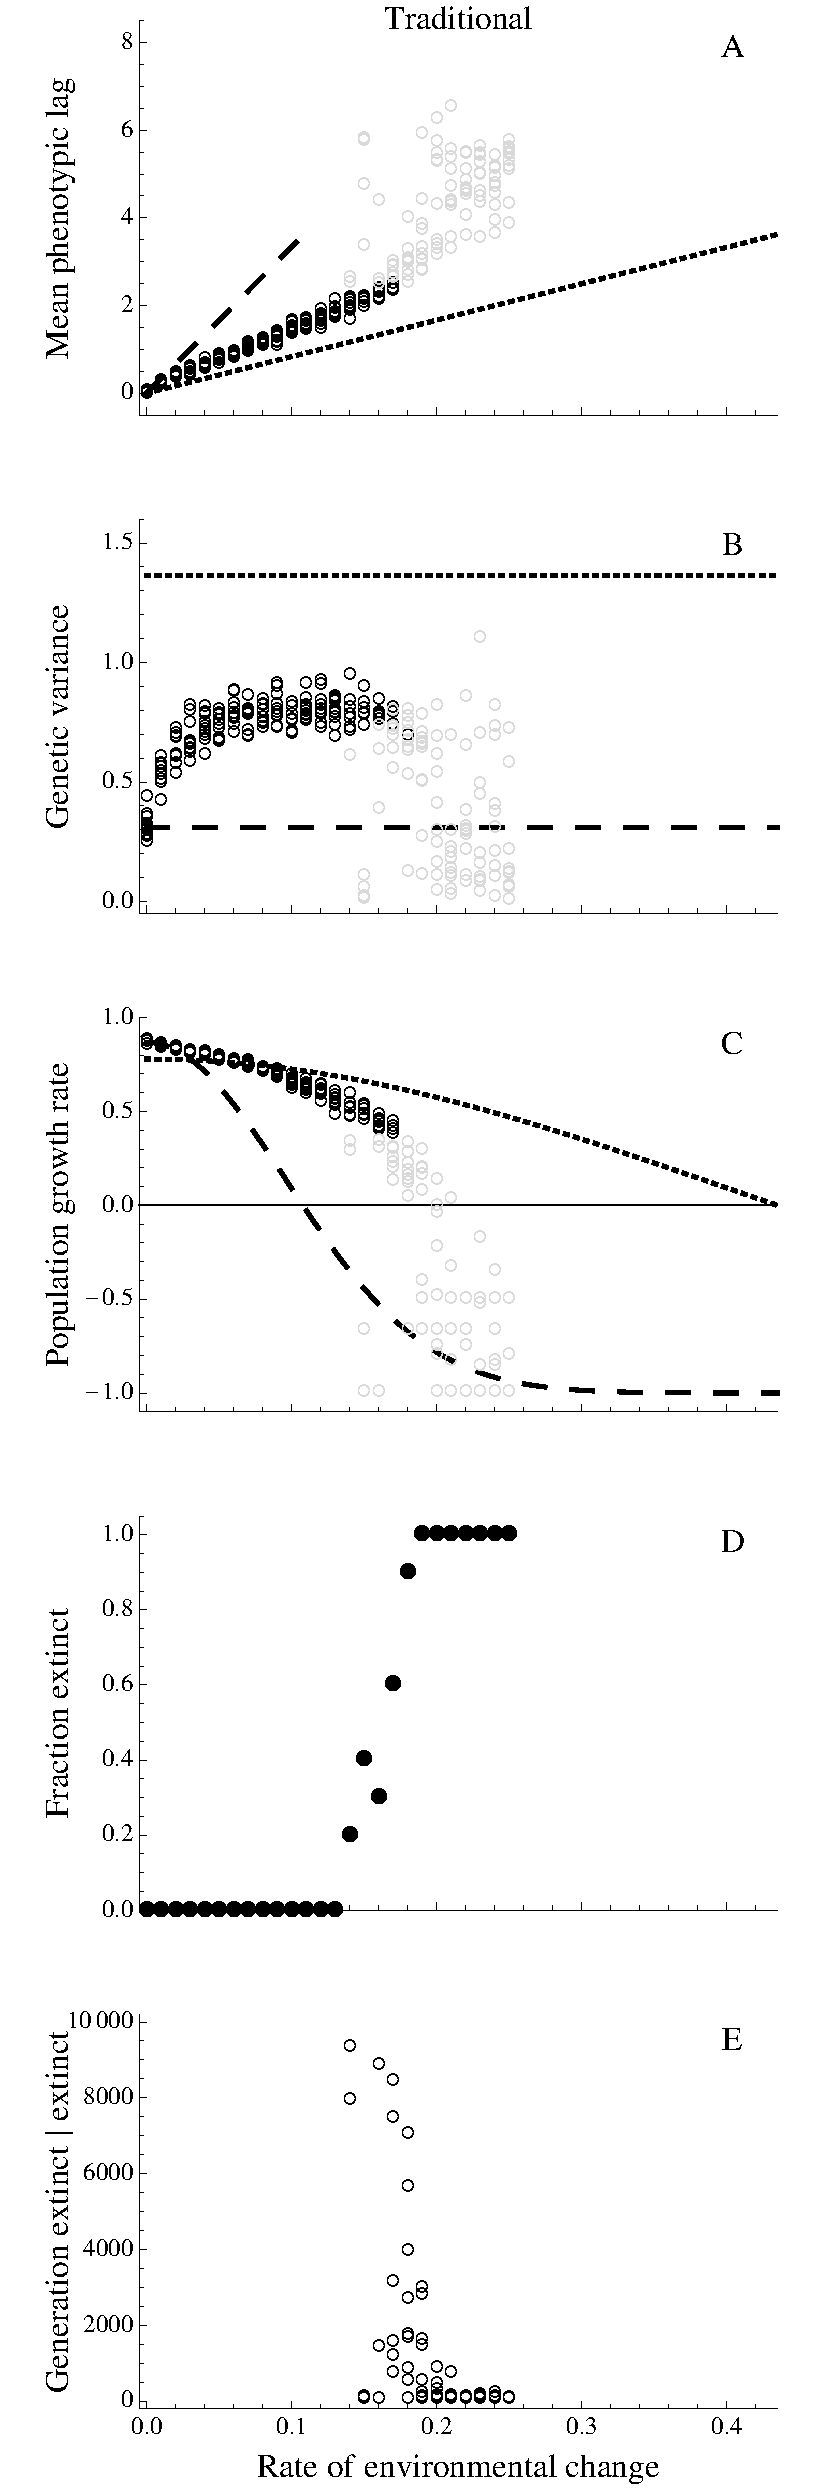
\includegraphics[width=0.45\linewidth]{IMAGES/TradSummaryMeanLargeBurn}
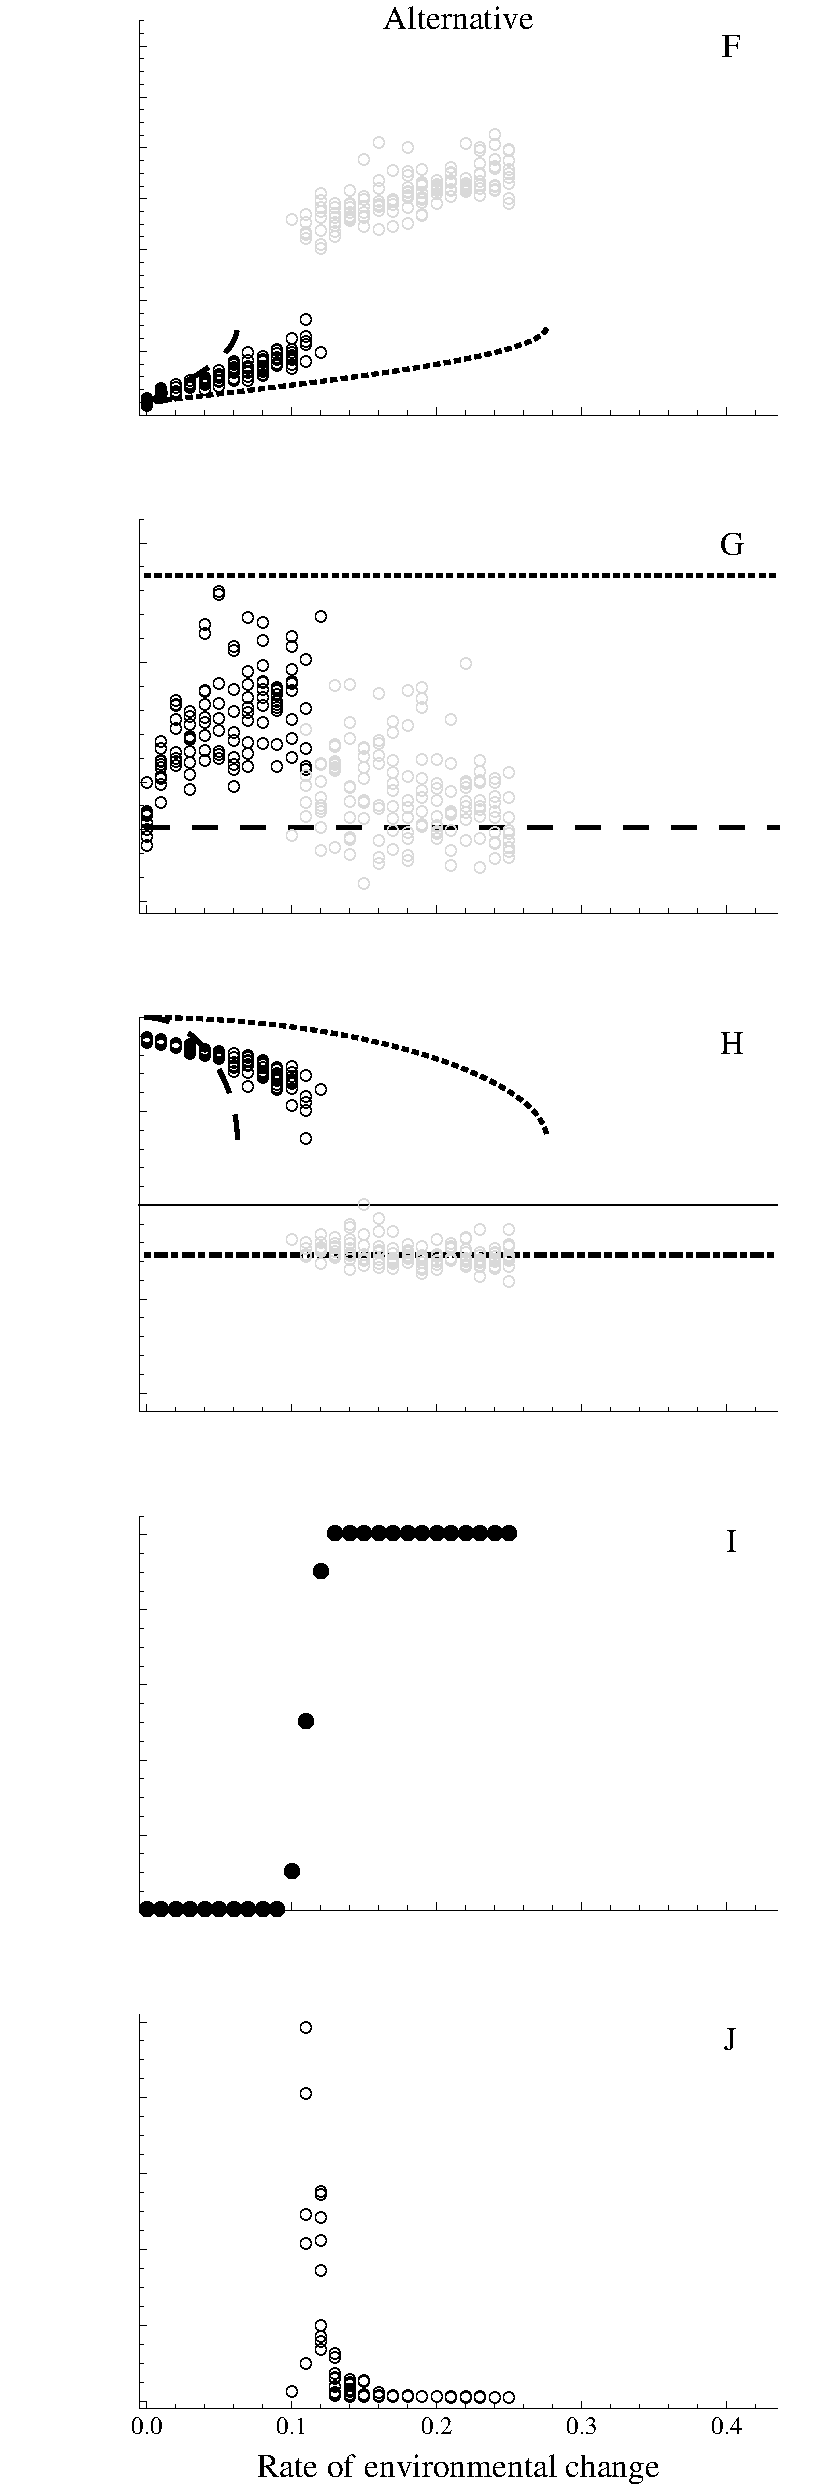
\includegraphics[width=0.45\linewidth]{IMAGES/AltSummaryMeanLargeBurn}
\caption{
}
\label{ModerateSummaryLast}
\end{figure}
%
%\begin{figure}[!ht]
%\centering
%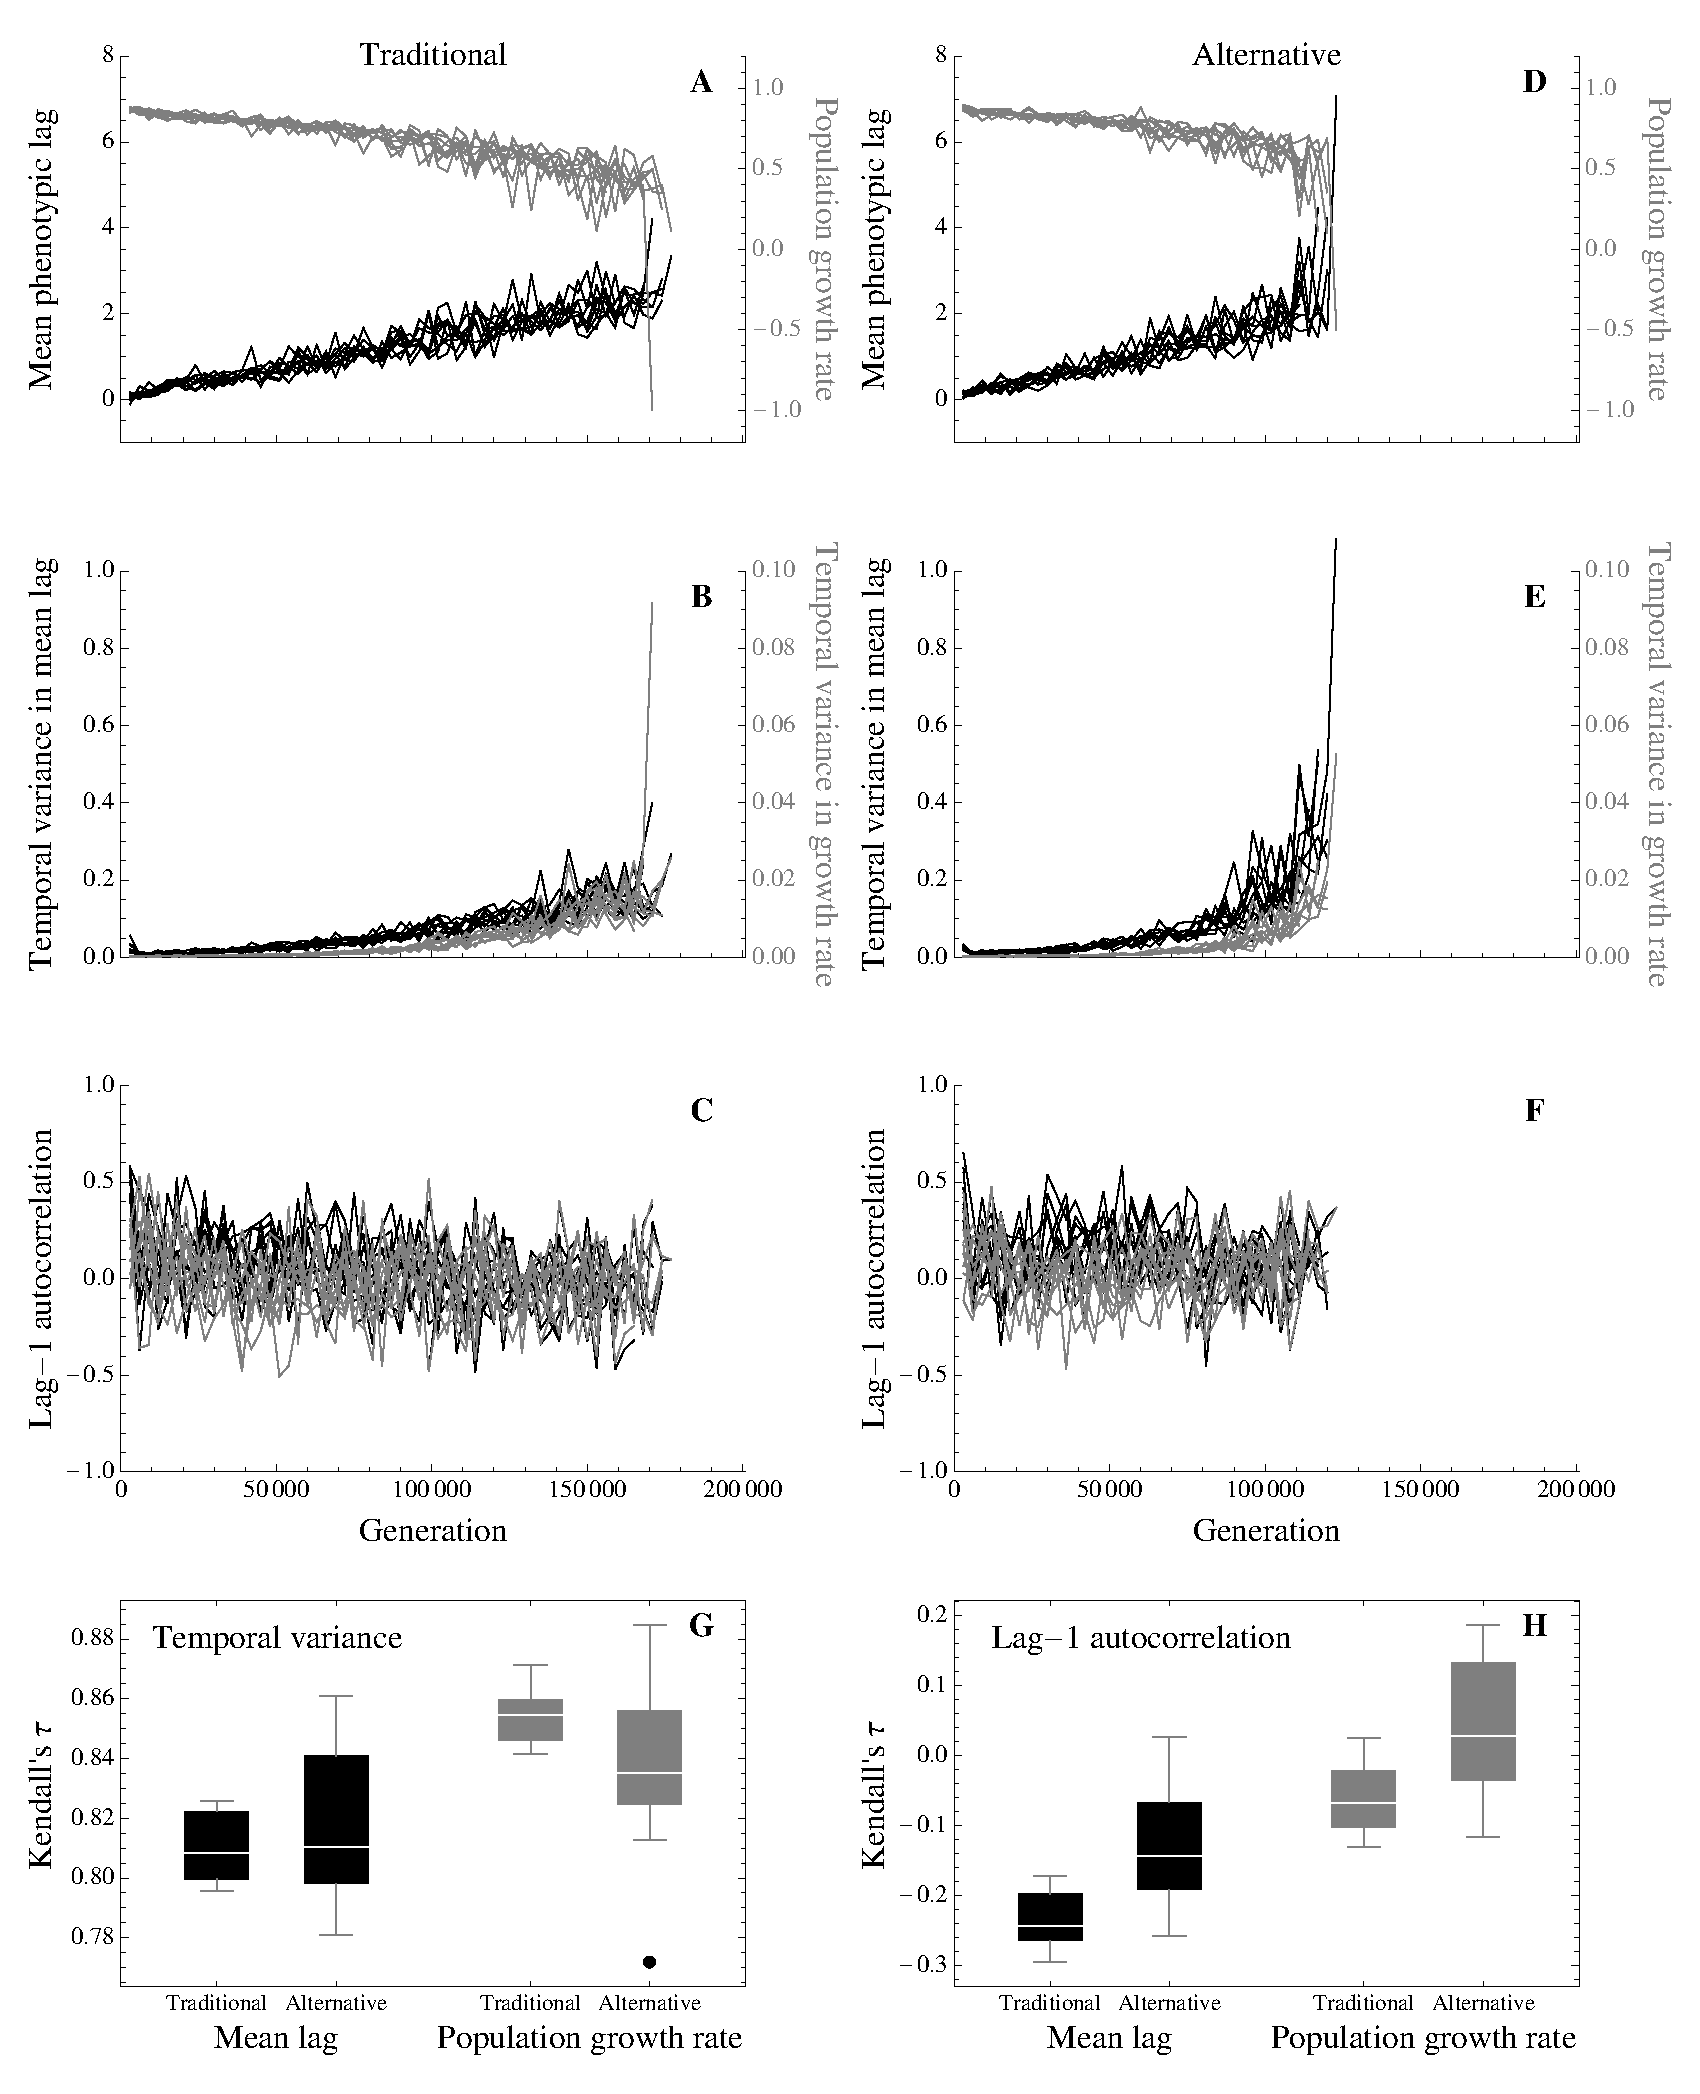
\includegraphics[width=\linewidth]{IMAGES/EarlyWarningSignsLarge.eps}
%\caption{
%}
%\label{ModerateWarnings}
%\end{figure}
%
%\begin{figure}[!ht]
%\centering
%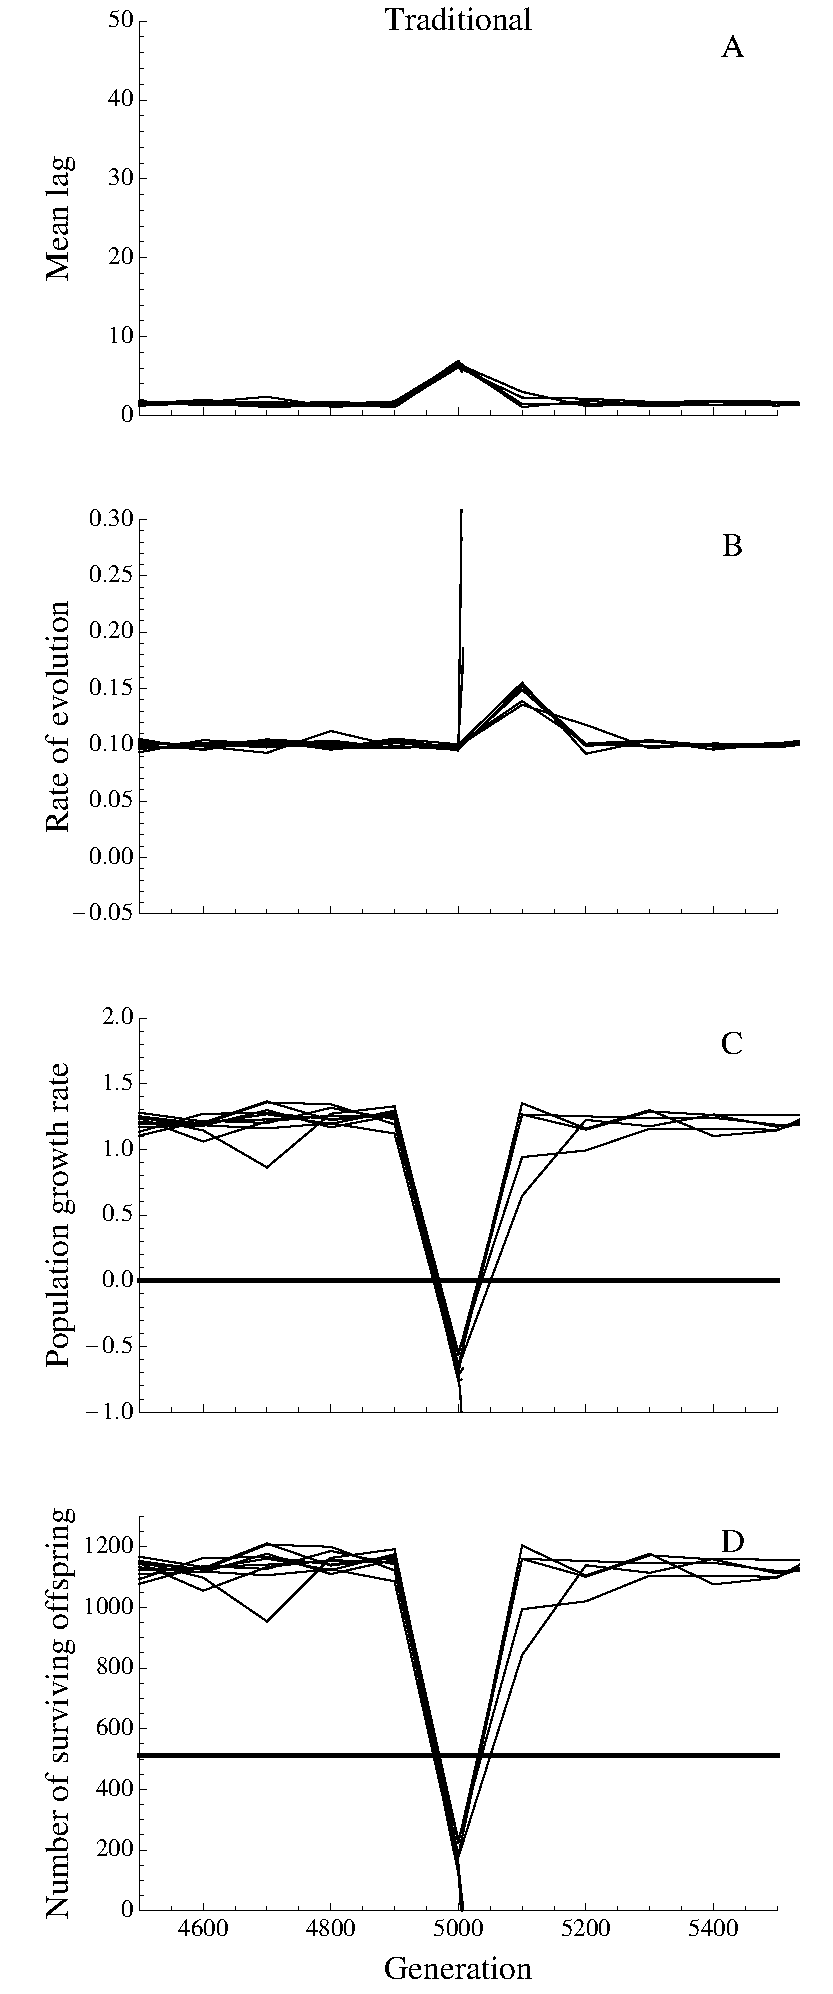
\includegraphics[width=0.45\linewidth]{IMAGES/TradHysteresisSnapshotLarge}
%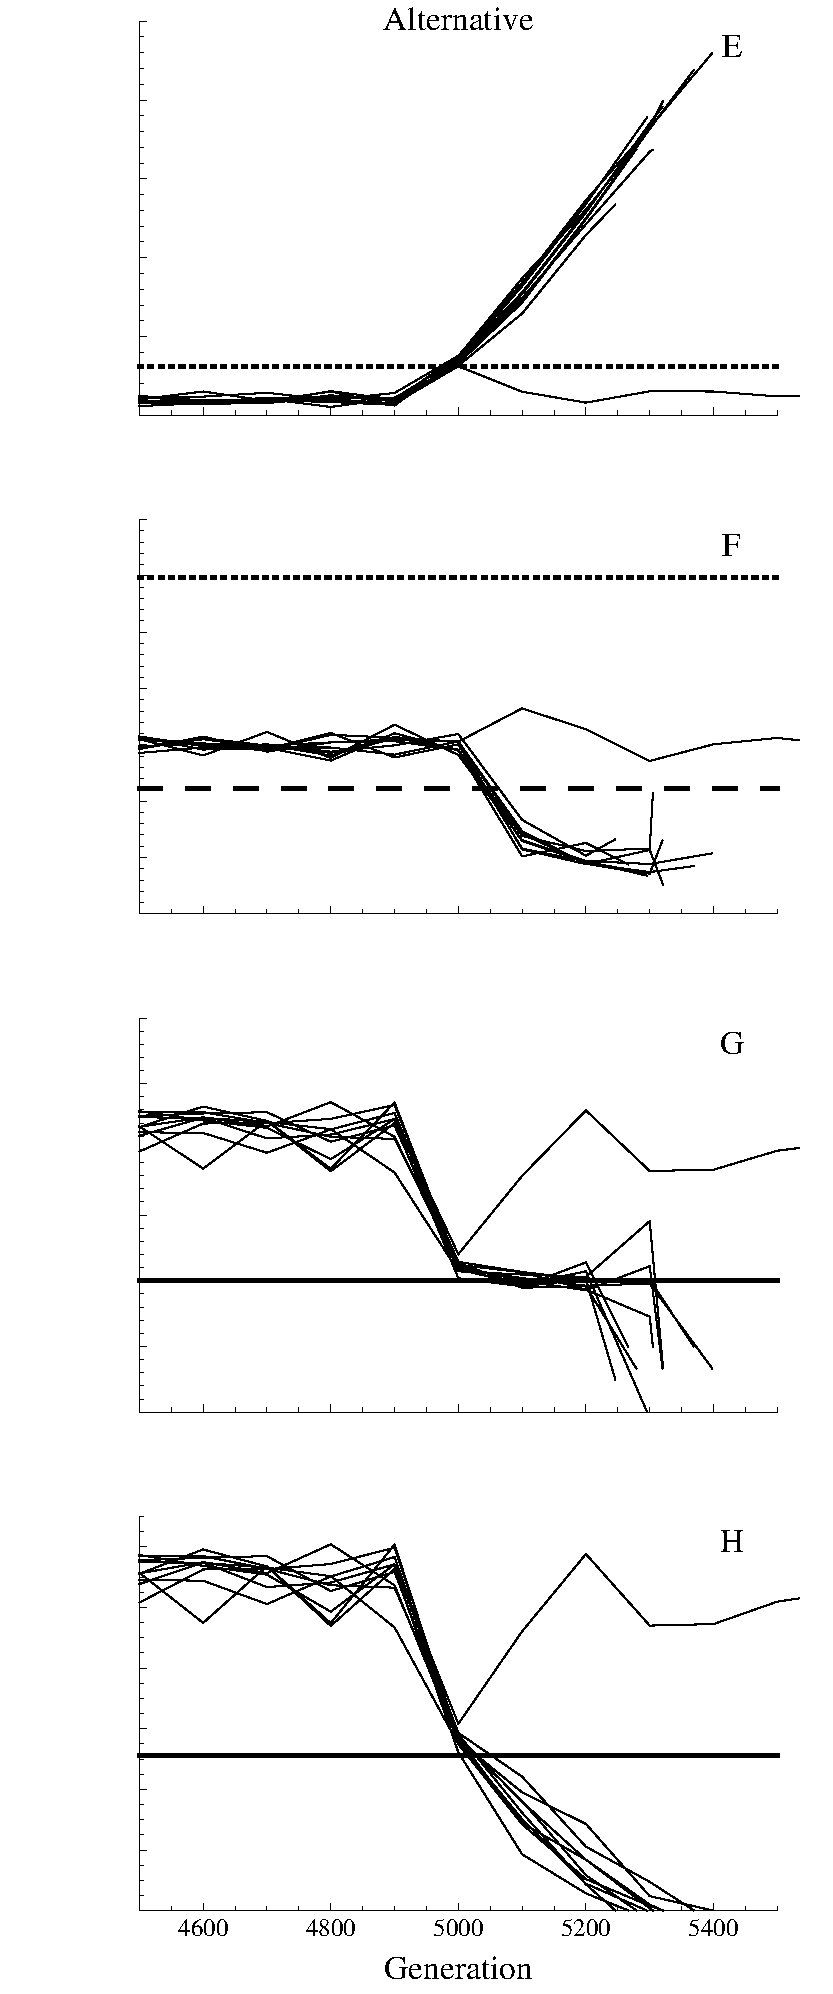
\includegraphics[width=0.45\linewidth]{IMAGES/AltHysteresisSnapshotLarge}
%\caption{
%}
%\label{HysteresisSnapshot}
%\end{figure}

\end{document}